\chapter{Related Work} 
\todo{write a paragraph about the commercial systems specially time domain and a paragraph explaining the table}
This chapter describes the overview of related research in the area of human being detection and tracking with UWB radar. First a background of human detection and tracking with UWB radar is presented then a short introduction of UWB radar system is given. Later signal processing steps and human radar cross section are explained briefly and at last the state of the art research in UWB radar for human presence detection and localization is presented. A summary table comparing signal processing methods, accuracy, hardware used and the measurement set up is shown in \ref{tabel: state of the art}.
\section{Background}
Human detection and tracking consists of measuring spatio-temporal properties of human such as presence, count, location, track and, identity \cite{Teixeira2010}. 
%properties of human are shown in figure \ref{fig:HumanSensing}.
%In safety application it is important that the machine slows down or stop when a person is getting too close to it therefore identifying the person is not needed.
Human measurable traits with UWB radar are shown in Figure \ref{fig:HumanDetectionWithRadar}. It is possible to measure reflectively of a human, some external motions such as walking and hand and feet movements, and some internal motions for example involuntary motion of internal organs such as heart beat and breathing with the UWB radar.
%Human detection with UWB radar can be divided into two categories: detection of humans through-wall (obstacles) and and detection of humans in Line Of Sight (LOS).
 %UWB radar is a better candidate than search dogs in rescue operations because search dogs can not differentiate between dead or alive people and can waste valuable time of the rescue team. In police raid operations the knowledge of criminals positions and number inside a building can bring valuable information to the operation \cite{Zaikov2008}, \cite{Li2012}.

UWB radar is used for human detection in Line Of Sight (LOS) \cite{Kilic2014,Shingu2008,Chang2009} as well as detection of people behind obstacles and walls because it has the capability to penetrate most building materials \cite{Sachs2008,Nezirovic2010,Rovnakova2013,Zetik}. This thesis focuses on detecting human beings in LOS with UWB Radar in cluttered environment like mines. 
%Through wall detection of humans have many applications such as rescue operations for example searching under rubble after earthquakes and surveillance in situations like police raid operations. 
 Through wall detection research is also reviewed as they contain the same algorithms and  techniques for human feature detection plus extra step of removing the clutter from the signal due to the existence of the obstacle or wall. The wall distorts the radar signature in form of attenuation, refraction, and multipath therefore the wall effect shall be compensated by using the known parameters such as thickness and relative permittivity of the wall. 


% \begin{figure}
%     \centering
%     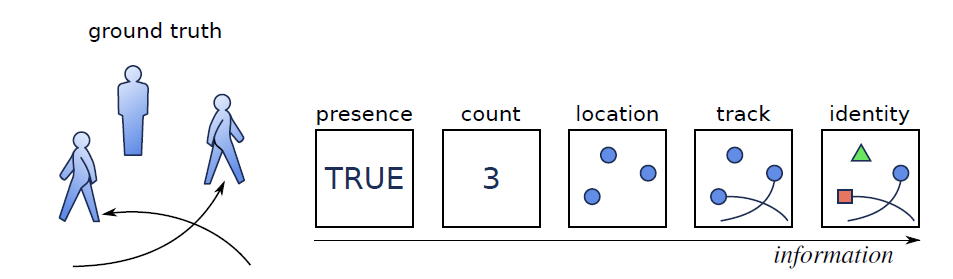
\includegraphics[width=\textwidth]{Figures/HumanSensing.PNG}
%     \caption{The Spatio-temporal properties \cite{Teixeira2010}}
%     \label{fig:HumanSensing}
% \end{figure}
\begin{figure}[t!]
  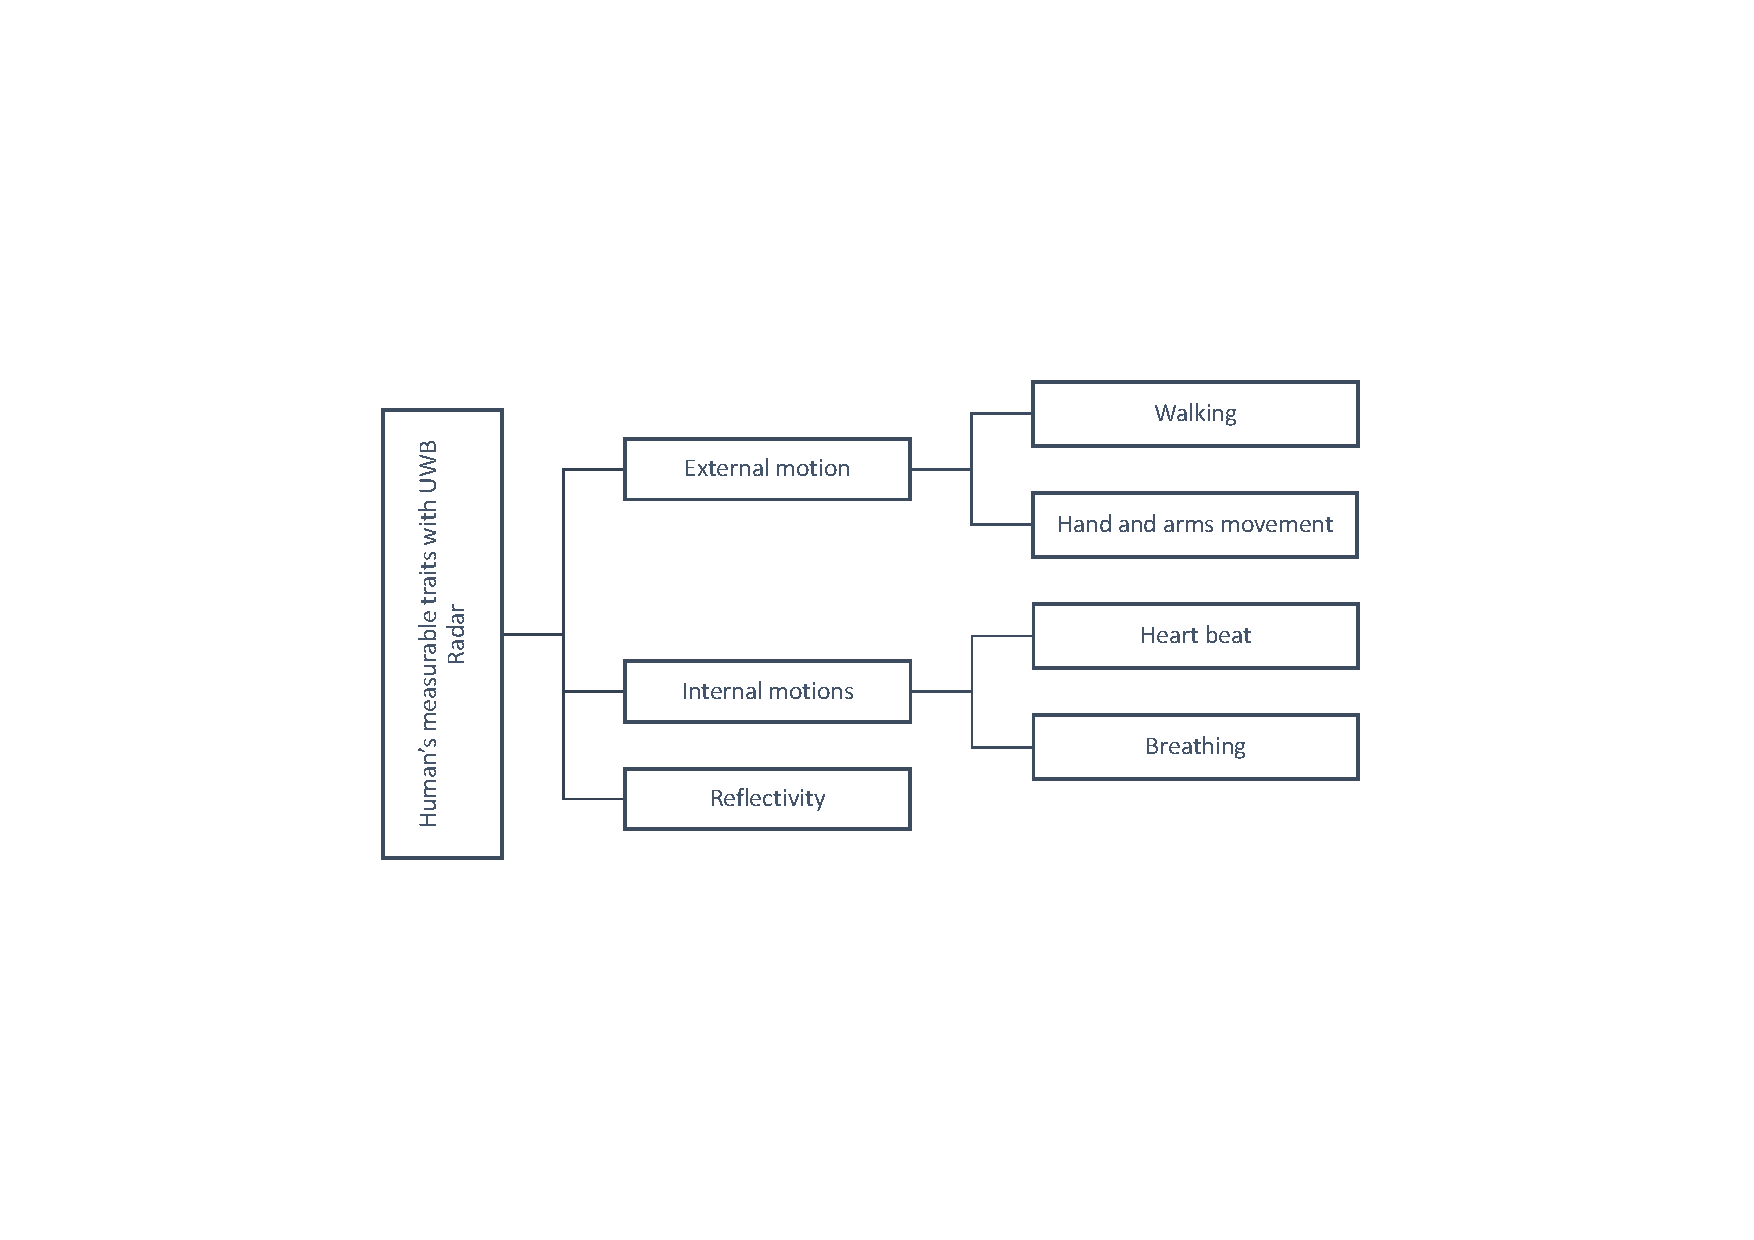
\includegraphics[width=\textwidth]{Figures/graph.pdf}
  \caption{Measurable Human traits with UWB radar}
  \label{fig:HumanDetectionWithRadar}
\end{figure}
% \begin{figure}
%     \centering
%     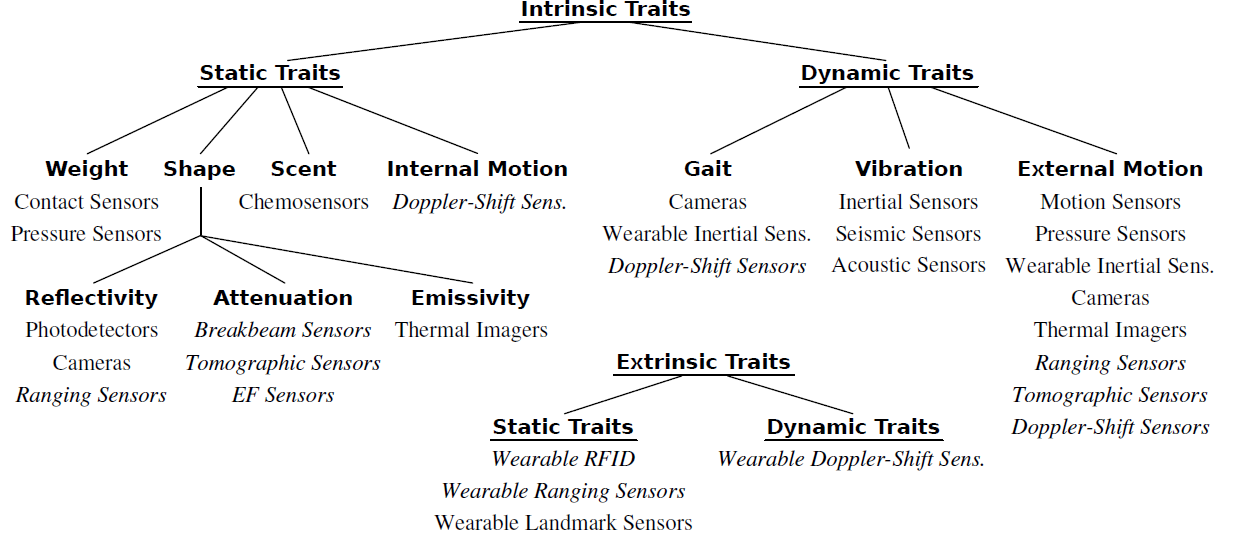
\includegraphics[width=\textwidth]{Figures/HumanTrait.PNG}
%     \caption{Taxonomy of measurable human traits \cite{Teixeira2010}}
%     \label{fig:HumanTrait}
% \end{figure}

\section{UWB Radar System}
Based on Federal Communications Commission (FCC) definition a signal can be defined as UWB signal if the fractional band with is greater than 0.2 where fractional bandwidth is defined in equation \ref{FracBW}.
\begin{equation}\label{FracBW}
	B_{f} = 2\frac{f_{H}-f_{L}}{f_{H}+f_{L}}
\end{equation}
% The first UWB signal was generated by Hertz in 1887. At that time that was the easiest way to create wave-forms. It was not until 1990 that the development in digital signal processing and invention of Time Hopping impulse radio in addition to the decision of U.S. frequency regulators to make frequency band between 3.1-10.6 GHz free for unlicensed operation of UWB devices awakened the interest for UWB radio \cite{WinHistoryUWB}.  
% The majority of traditional radar system are based on a narrow band signal modulated on a sinusoidal carrier wave and due to limited bandwidth the amount of information that they can carry is limited. By using a narrower pulse in order of nanoseconds in Wide band and UWB systems the accuracy of target range and the ability to detect smaller targets is increased which in turn increases the radar resolution. This will result in better identification of the target. In addition it will reduce the passive interference from for example rain and other particles due to relative reduction of scattering cross section of interference to the target. It also increases immunity to other narrow-band sources \cite{Taylor2000} and \cite{ImmoreevUWBAdvantage}
%why UWB is better that other radar systems

% Some active localization system require the person carry a radio-frequency tag
% The disadvantage is that the data is not possible to be visualized for a human eye contra vision system
% detection relies on the back-propagation of the signal from the body
% Creating signals with a large bandwidth can be achieved in many different ways such as Frequency Hopping (FH), Time Hopping (TH) and Direct Sequence (DS) or allow modulation schemes to work at extremely high data rate such as Orthogonal Frequency-Division Multiplexing (OFDM) \cite{WinHistoryUWB}. 
Different types of UWB radar are developed and based on the excitation wave-form\todo{give some references} they are divided to different categories. Three of the most prominent categories are Frequency Modulated Continuous Wave (FMCW), pulse and, M-sequence. In this research we have access to a commercially available M-sequence UWB radar which is developed in Radarbolaget (G\"{a}vle, Sweden). Radarbolaget is developing radar systems primarily for real time, through wall monitoring of heating furnaces\footnote{http://www.radarbolaget.com}.

\subsection{Ultra Wide-band Antennas}
An UWB system requires an antenna capable of receiving all the frequencies at the same time. Thus, antenna behavior and performance must be consistent and predictable across the entire band. Ideally, pattern and matching should be stable across the entire band and the antenna shall be preferably non-dipersive and have a fixed phase center \cite{SchantzUWBAntenna}. Furthermore the frequency-dependent characteristics of the antennas and the time-domain effects and properties have to be known \cite{WiesbeckUWBAntenna}.

There are different types of UWB antennas which are used in UWB systems such as  traveling-wave structures, frequency-independent antennas,  multiple resonance antennas, and electrically small antennas.
In this project a pair of Vivaldi antennas developed in the University of G{\"a}vle are used in the radar system.\todo{I don't understand what should I explain here} The Vivaldi antenna guides the wave from the feed in a slot line to the exponential wide-band taper which radiates all the frequency under proper radiation condition. The taper shape can be designed so it provides a smooth transitions. The Vivaldi antenna has relatively low distortion compared to other UWB antennas. 
\todo{picture of radars?}
%In \cite{Nanzer2017} Nanzer has reviewed the microwave wireless techniques for human presence detection and classifying human activities and discusses prominent examples of experimental systems from the literature. The types of radars used for human presence detection are firstly introduced. Later a review of remote biometric measurements, focusing on respiration and heart rate is presented . Finally, passive radiometers methods for human presence detection are introduced

\section{Signal Processing}
To be able to extract the human target signal, raw radar data passes several signal-processing steps. This signal usually is affected by noise, clutter and attenuation. %In UWB radar based systems signal processing is done in the time domain rather than frequency domain therefore some of the traditional signal processing algorithms.
In \cite{RovnakovaSignalProcessing} UWB radar signal processing steps is described that are shown in Figure \ref{fig:SignalProcessing}.
\begin{figure}
  \centering
  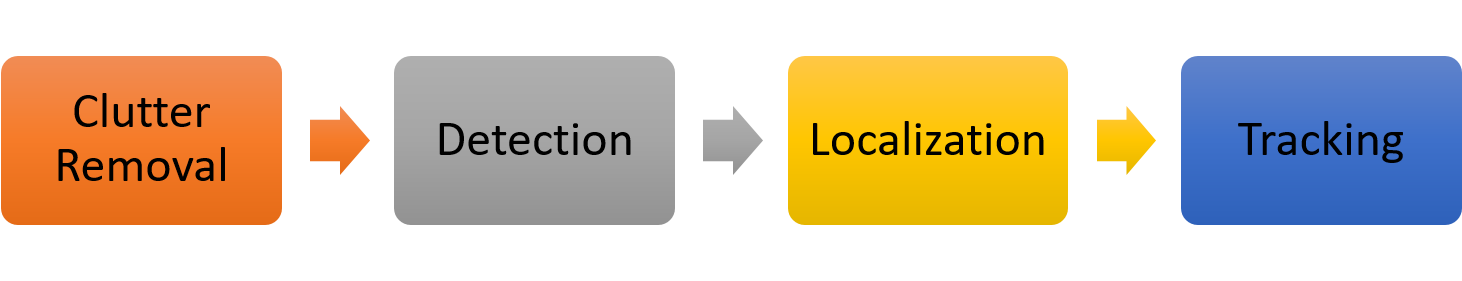
\includegraphics[width=\textwidth]{Figures/SignalProcessingSteps.png}
  \caption{UWB Radar Signal Processing Steps}
  \label{fig:SignalProcessing}
\end{figure}

\subsection{Clutter Removal}
Clutter is unwanted radar return signals. The focus of this thesis is on human detection in highly cluttered environment like mines so the effect of clutter on signal detection needs to be investigated. Clutter contains the antenna cross-talk (A direct wave propagating from the transmitter antenna Tx directly to the receiver antenna Rx) and waves reflected from other objects except the human in the scenario such as walls and machineries. Sources of clutter can be out-of-band interference which contains frequencies other than dedicated bandwidth for the system or in-band interference and thermal noise. Out-of-band interference can be detected and removed by traditional techniques such as Fourier transform and band-pass filter. In-band interference is harder to identify and to remove. Clutter can affect the probability of detection and accuracy. To understand and quantify clutter the statistical properties of the clutter are often used. A statistical radar clutter model for modern high resolution radars is presented in \cite{clutterModel}. Densities such as Weibull or log-normal distributions are shown to provide reasonable fits for measured clutter densities. In equation [\ref{eq:LogNormal}] the Probability Density Function (PDF) of log normal distribution is shown.
\begin{equation}
f_X(x;\mu,\sigma) = \frac{1}{ x\sigma \sqrt{2 \pi}}\, e^{-\frac{(\ln x - \mu)^2}{2\sigma^2}},\ \ x>0
\label{eq:LogNormal}
\end{equation}
where $\mu$ and $\sigma$ are the mean and standard deviation of the variable x natural logarithm respectively.
 Clutter removal techniques could have different complexity based on application, speed, accuracy, and, memory requirement. One common method concerning detection of static objects is background removal. A measurement of the background before the object is placed in radar vicinity is removed from the raw radar data after the object is placed in the radar vicinity \cite{BryanClassification}. This method has a drawback because it does not consider the shadowing phenomena i.e. the existence of the static object will change the reflection from all the other static objects in the scene. It simply means Background and static object - background $\neq$ static object.

Exponential averaging is another clutter removal method used when dealing with a moving object. Exponential averaging has advantages such as low complexity and good performance \cite{Zetik}. In this method, the clutter estimated from the previous radar sweeps and updates is removed from the actual radar measurement at the moment.
\begin{equation}
S_{t} =\alpha .Y_{t} + (1-\alpha).S_{t-1}
%\label{eq:ExpoAver}
\end{equation}
Where $\alpha$ is a coefficient between 0 and 1, $Y_{t}$ is the signal and $S_{t}$ is the exponential average at time t. $S_{1}$ can be set to the first signal value. 

\subsection{Detection}
To differentiate between a human and other objects or artifacts such as antenna cross talk is a challenging task. The transmitter and receiver antennas are located closely to each other so the cross-talk power is relatively much greater than the reflection of a human body standing at several meters from the antennas. Based on Figure \ref{fig:HumanDetectionWithRadar} the human can be detected either by the motion or reflectively. The algorithms such as micro-Doppler can detect periodic motions such as movement of arms and legs or breathing. If there are other moving objects in vicinity of the radar the detection will be more demanding and there will be a need to object recognition afterwards.
An UWB radar provides high-resolution range profile as well as high resolution Doppler spectra. Doppler signature of the human by UWB radar is shown in \cite{WangUWBDopplerPhD}.

% \begin{figure}
% \centering
%   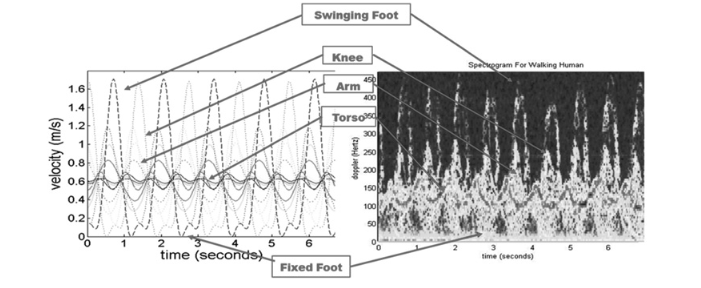
\includegraphics[width=\textwidth]{Figures/Microdoppler.PNG}
%   \caption{Modeled human velocities compared to a measured spectrogram of a man walking towards radar \cite{TahmoushUGS}}
%   \label{fig:MicrodopplerHuman}
% \end{figure}
Detection step is about making a decision between if the signal scattered from target is absent or present in radar data. One the solution is using statistic theories to test the suggested target against a threshold. The result of this decision is a binary data where 1 means that the target is probably present in the radar scan and 0 indicates the lack of target. For UWB radar detection problem fixed threshold, (N,k) detectors, IPCP detectors and constant false alarm rate detectors (CFAR) is proposed \cite{TayloUWBTech}.

\subsection{Localization}
Time Of Arrival (TOA) of the detected target is the time that it takes for the wave to travel from the transmitter to the target and scattered back again to the receiver. The distance to the target is calculated by equation \ref{eq:TOA}.
\begin{equation}
\label{eq:TOA}
	\textnormal{Distance to the target} = \frac{TOA * C}{2}
\end{equation}
where C is the speed of light.
%For 3D position estimation in a coordinate system at least 4 anchor nodes are needed otherwise the ambiguity in position estimation will occur.
Position estimation methods can be divided into two categories: iterative and non-iterative methods \cite{Shen2006}. Direct Method (DM) \cite{KegenYu}, Least Square (LS) \cite{YitengHuang2001} and Spherical Interpolation (SI) \cite{Schau1987} are some of the non-iterative approaches to solve position estimation problems. Taylor Series method is an example of iterative approach for localization \cite{FOY1976}.

\subsection{Tracking}
Tracking algorithms are often used to increase the precision of the localization results for moving targets. Most of the tracking algorithms can make an educated guess about target's next position and reduce the measurement's uncertainty and smoothen the target trajectory. Kalman filter, linear least square and particle filter are widely used in this application \cite{Denis},\cite{Sobhani2014}.

\section{Human Radar Cross Section}
To be able to quantify target echo in terms of  the target characteristic, a term called Radar Cross Section (RCS) is defined. The RCS is the projected area of a metal sphere that would return the same echo signal as the target.
Radar cross section depends on many factors such as frequency and polarization of incident wave and the target aspect (its orientation relative to the radar). Calculation of RCS is a matter of finding the scattered electric field from the target which it means to calculate the induced current on the target by solving Maxwell's equations for complicated boundary conditions which usually is solved with numerical methods.
% %%%%%%%%%%%%%%%%%%%%%%%%%%%%%%%%%%%%%%%%%%%%%%%%%%%%%%%%%5
% LOS human detection 
%%%%%%%%%%%%%%%%%%%%%%%%%%%%%%%%%%%%%%%%%%%%%%%%%%%%%%%%%%%5
\section{State of the Art}
\todo{A summary table would be included in here}
% \begin{table}
%   \centering
%   \caption{State of the Art}
%   \label{tabel: state of the art}

% \begin{adjustbox}{width=\textwidth,angle=90}
%     \begin{tabular}{l|l|l|l|l|l|l|l|l} 
%     \hline
%     Author & Background subtraction & detection & Case(wall or not) & Hardware & Distance  & Antenna & Localization& Tracking
%     \\\hline
%     Chang2009 &	MTI & MTT and hypothseis testing &	LOS, differentiate between cars and human &	PulsOn 210& 0.3 -12.2 m& Time Domain	& TOA	& multi-target tracking (MTT)\\

%     \hline
%     \end{tabular}
% \end{adjustbox}
% \end{table}
%\csvautotabular{tabel.csv}
\begin{sidewaystable}
    \centering
    \caption{State of the art for human being detection with UWB radar, NA stands for Not Applicable}
    \label{tabel: state of the art}
    \small
\begin{tabularx}{\textwidth}{|p{1.7cm}p{1.7cm}p{1.7cm}p{1.4cm}p{1.3cm}p{1.2cm}p{1.2cm}p{1.5cm}p{1cm}|}
%{|*{9}{>{\RaggedLeft\arraybackslash}X|}}

\hline
    Author & Background subtraction & Detection & LOS/NLOS & Hardware& Distance & Antenna & Localization& Tracking
    \\\hline
    \rowcolor{Gray}
    Chang et al.\cite{Chang2009} &	MTI & MTT \& hypothseis testing &LOS &Time Domain\textsuperscript{TM}& 0.3–12.2m& Toroidal Dipole	& TOA	& MTT\\
    
    Kilic et al. \cite{Kilic2013}&Averaging&Likelihood test&LOS&Time Domain\textsuperscript{TM}&1m-4m&Toroidal Dipole&Threshold crossing criterion&NA\\
    \rowcolor{Gray}
    Rane et al. \cite{RaneMovintargetUWB}&	Band-pass filter \& Range profile subtraction	& peak of STA/LTA &LOS, behind concrete wall and wooden door& Time Domain\textsuperscript{TM}&6m& Toroidal Dipole&STA/LTA&NA\\				

    Sachs et al. \cite{Sachs2008} &	High-pass adaptive filtering &	CFAR &	LOS and under rubble & M-sequence & 17m& Spiral &	CFAR &	NA\\
    \rowcolor{Gray}
    Zetik et al. \cite{Zetik} & Adaptive exponential averaging & NA & Behind wall & M-sequence&	NA&		Horn&	TOA & NA\\
    
    Ossberger \& Buchegger \cite{OssbergerRespiratory} & Removing average &	Wavelet transform &	LOS& Pulse generator & 	1-5m &	Horn & NA& NA\\
    \rowcolor{Gray}
    Nezirovic et al. \cite{Nezirovic2010} &	Linear least-squares &	RMD, SVD &	Pile of bricks and a concrete pipe&	 M-sequence & 1.6m & Horn&NA&NA\\			
    
    Rova\v{n}kov\'{a} and Kocur \cite{Rovnakova2013} & Exponential averaging & CFAR &	Behind wall& M-sequence  & Max 3m& Horn& TOA &	Kalman Filter\\
    \rowcolor{Gray}
    %Maaref et al. \cite{PichotFMCWUWB}&&&&&&FMCW&&\\
    
    Shingu \cite{Shingu2008}&	NA&	Maximum amplitude&	LOS&	Network Analyser&	Max 6m	&Horn&	TOA&NA\\
    Zhao et al.\cite{ZhaoHMM}& NA & HMM&	Gypsum wall and wooden door&	Time Domain\textsuperscript{TM}&6.5 feet, 7.5 feet&	Toroidal Dipole&NA&NA\\
    \hline

\end{tabularx}
\end{sidewaystable}

In \cite{Chang2009} Chang et al. are addressing the problem of providing pedestrian safety in the presence of moving vehicles by using an UWB impulse-based mono-static radar. A specular multi-path model (SMPM) is used to characterize human body scattered UWB waveforms to detect the presence of humans via gait. The SMPM is a computationally useful signal representation that reduces UWB waveform representation to 2 dimensions (path amplitude and TOA). First the moving target indication (MTI) system which rejects highly human-unlike stationary clutter. Then the CLEAN algorithm is applied to the MTI response of radar scan to obtain estimated TOAs and amplitudes of the decomposed multipath components, then the signal is segmented in time to isolate the scatters associated with individual moving objects, then each segment is be associated to segments from previous recording intervals with the aid of a multi-target tracking (MTT) technique. Then a hypothesis testing process determines whether the tested track is interpreted/detected as a human or not based on three features:(1) the path’s maximum magnitude, which is relevant to target composition and cross-section size; (2) the RMS delay spread of multipath delay profile (or the RMS range spread), which is relevant to target size over the range dimension; and (3) the velocity of target. This approach is tested in a realistic outdoor environment and shows better than 80\% detection probability with 1.58\% false alarm rate.

In \cite{Kilic2013} Kilic et al. present a technique for detection of static humans based on the fact that a human presence induces small low-frequency temporal variations in UWB signal that stand out against the background signal. The experiment is performed in indoor environment where 3 radios are installed as anchor nodes and the person is standing in 48 different places with 50 cm in between every position. To remove unwanted background, signals averaged over time, and then  the averaged signal is subtracted from the raw signal. Later a likelihood test determines if the human exist in vicinity of the radar. To locate the person two different methods were tested: Line search and Threshold Crossing. Line search is simply search the maximum value in the signal. In some conditions largest peaks does not always corresponds to the person, especially if the person are close to strong reflectors.\todo{this sentence shall be revised} In this case, not only the paths that are directly reflected off the person, but also the indirect reflections show fluctuation over time. For that a threshold-based method is purposed. The results were examined in terms of missed detection and accuracy.  Depending on the fractional bandwidth and measurement duration the missed detection rate changes between 0.02 and 1. The accuracy is reported less than 65 cm. Proposed technique could be also applicable to cases with multiple people.

%%%%%%%%%%%%%%%%%%%%%%%%%%%%%%%%%%%%%%%%%%%%%%%%
%Behind obstacle
%%%%%%%%%%%%%%%%%%%%%%%%%%%%%%%%%%%%%%%%%%%%%%%%
Human detection behind walls is the dominant subject in UWB research area. 
In \cite{RaneMovintargetUWB} Rane et al. purposed a Short Term to Long Term Average ratio (STA/LTA) to detect moving target by UWB radar behind obstacles. The method is based on enveloping the signal by Hilbert transform and averaging. The results show that this method shows 79.6\% more accuracy than choosing the simple peak of processed range profile to estimate the distance. For pre-processing IIR bandpass filter of order 20 and passband of 3.1-5.3 GHz is applied along fast time dimension to suppress frequencies beyond the radar operating range. Stationary clutter is suppressed by performing weighted Range Profile Subtraction (RPS) on each range profile.
\todo{kilic and rane are not revised}
Sachs et al. in \cite{Sachs2008} used a M-sequence UWB radar with 3-antenna configuration (one transmitter and two receiver antennas) to detect moving people and trapped people under rubble. For moving people detection, the first signal processing step consists of removing the clutter caused from static objects by high-pass adaptive filtering. In the second step, CFAR processing for target indication and the corresponding TOA. Outliers and missing points are then removed and finally, the target trajectory is calculated. The paper concludes that the 3-antenna configuration is not robust against ghost targets by its principle. To detect trapped people under rubble the small movements such as breathing is out of interest. The signal can be enhanced by narrowband filtering carried out by applying a horizontal FFT on the data after clutter removal. Additionally, a sliding average with a short window was performed over the transformed signal in the propagation time direction. The experiment could detect the breathing person lying in a cement pipe.
%%%%%%%%%%%%%%%%%%%%%%%%%%%%%%%%%%%%%%%%%%%%%%%%
%Breathing
%%%%%%%%%%%%%%%%%%%%%%%%%%%%%%%%%%%%%%%%%%%%%%%%
%When the human is static the breathing activity hearth beat will be monitored and it will be mistaken for a static background and will be removed. 
In \cite{Zetik} Zetik et al. describe architecture and design of an M-sequence UWB through-the-wall radar for detection and localization of people. For background subtraction an adaptive subtraction method is purposed. This method is based on the exponential averaging although instead of a scalar weighing factor $\alpha$ vector of weighing time-variant coefficients ${\alpha}_k$ is introduced. The location of the target is measured by TOA. The achieved precision is in an order of 40cm.

In \cite{OssbergerRespiratory} a Continuous Wavelet Transform for detection of respiratory activity thorough wall with an UWB impulse radar test set-up is presented. CWT is suitable for non-stationary signals like pulses. It has been shown that the UWB radar can detect breathing up to 5 meters.

Nezirovi\'c et al. \cite{Nezirovic2010} present a Respiratory Motion Detection (RMD) algorithm. The algorithm is based on an RMD algorithm presented in \cite{Sachs2008} and complementing it with singular value decomposition (SVD). The purpose of applying SVD is to separate the respiratory motion response from the non-stationary clutter, and, in addition, reduce the effect of the Additive White Gaussian Noise (AWGN). A linear least-squares fit is purposed to remove stationary clutter along with any potential linear trend in the slow-time dimension. The results compares the developed RMD with reference RMD. The performance of the RMD algorithm is assessed both by means of a Monte Carlo simulation as well as experimental data acquired under realistic conditions of a person lying in concrete pipe under 1.2 meter bricks and moist soil. The results show increase in performance of the developed RMD algorithm over the reference RMD algorithm in terms of its de-noising capabilities and non-stationary clutter separation.

In many UWB applications the character of target motion is not known but usually signal processing algorithms aim at only moving persons or only static persons. In \cite{RovnakovaSignalProcessing} Rova\v{n}kov\'{a} and Kocur purposed a method to detect human behind walls which combines the moving and static person detection. Both detection methods are quite similar in signal processing procedures. To remove the background, exponential averaging method is used because of its robust performance and low complexity. For detection stage for moving clutter the CFAR detector is purposed. TOA is used to localize the target and  Multiple target tracking (MTT) system using a linear Kalman filtering used for target tracking.
For the static person, in order to further improve the signal-to-noise ratio of a static target echo, the impulse response with subtracted background is applied to a range filter which can reduce the clutter residue and noise. Additionally, breathing as a narrow band process can also be enhanced by the use of low-pass filtering. To extract the breathing rate, a horizontal Fast Fourier Transform (FFT) is applied.
A procedure for positioning of a person with unknown or changing motion activity is purposed. The performance of combined procedure is demonstrated by an experiment with one static person and one moving person changing his motion activity during the measurement. The results shows that it is possible to obtain more extensive and precise information about the position of monitored persons at the expense of computational complexity and time consumption.

%In \cite{PichotFMCWUWB} an UWB FMCW radar is used to detect human behind walls. First a simple model of the wall is introduced to model the wall response to radar waves. The transmission measurement is carried out to validate the wall model. A simulation is presented to present the human target in different distances from radar. An experiment is performed by someone walking behind a brick wall. The results show that it is possible to detect human targets behind obstacles with this method.


% Detection algorithms for UWB radar are discussed in \cite{Taylor2000}. Common solution to detection problems are (N,K)-detector \cite{VanDerSpek1971}, the interperiod-correlation processing (IPCP) detector \cite{Immoreev} and the constant false alarm rate (CFAR) detector\cite{Kapoor1999}.

% %%%%%%%%%%%%%%%%%%%%%%%%%%%%%%%%%%%%%%%%%%%%
% \cite{RangeDopplerHe} uses double canceler (3-order moving target indication filter) is considered to be suited to this application due to its simplicity and efficiency
% %%%%%%%%%%%%%%%%%%%%%%%%%%%%%%%%%%%%%%%%%%%%%%%

% \todo{use a good picture to show how radar data is comming out}

% %%%%%%%%%%%%%%%%%%%%%%%%%%%%%%%
 In \cite{Shingu2008} Shingu et al. studied human being existence detection and localization with simulation of an UWB radar sensor network. Akaike Information Criterion (AIK) to judge the approximate of the amplitude distribution of the received power of human body. It is concluded that Gaussian distribution is the best fit as a clutter model. The simulation results are compared with real propagation measurement with the network analyser. The localization error is shown to be 14 cm or less.
% %%%%%%%%%%%%%%%%%%%%%%%%%%%%%%%

Radar returns from human with motions are subject to Doppler modulations that provide
information about motion dynamics. In \cite{VChenHuman} V.Chen discusses the radar back-scattering from a walking human model and based on the model a motion trajectory and velocity pattern of human body part is derived. Then the time-frequency transform of the signal is analyzed to derive the micro-Doppler signature of human movement and complex arm and motion movements are analyzed. The micro-Doppler signature of the complex arm and leg motions are characterized.

He et al. in \cite{RangeDopplerHe} examined the feasibility of using range Doppler processing with multi-static UWB radar in tracking of humans behind walls. Range-Doppler (RD) processing is using Doppler effect to determine the radial effect of target velocity. The advantage of using RD is to resolve multiple targets not only in range but also in Doppler. To achieve better Doppler resolution for high range-resolution radar a range mitigation compensation algorithm is purposed. A measurement with m-sequence pseudo-noise radar is performed and the range migration compensation shows a better result both is Doppler and range profile.
\newline
Micro-Doppler effects has been studied in through wall applications. In \cite{RamMicrodopplerThroughWall} the simulation showed that the wall introduces minor distortion on micro-Doppler effect of human body parts but it affects the magnitude response of Doppler effect in form of attenuation and fading. The experiment is based on a Doppler radar but the preliminary investigations by the authors shows that the same methodology can be applied to a wide band radar. 
% In\cite{SChangUWBHumanDetection} S.Chang et.al used a database to record features in radar return such as cross section size and velocity of the target and used this database to to classify human targets. 
% In \cite{MicroDopplerGaitTahmoush} D. Tahmoush and J. Silvious extract the radar micro doppler signals generated by human motion and extract of gait features from it.
% localization and tracking with radar sensors can be device free or with active or passive tags 
\newline
 In \cite{ZhaoHMM} Hidden Markov Model(HMM) is used to classify the target in presence of clutter. The experiment is done in two scenarios: a scenario with dense foliage and a 1.5 meter trihedral metal reflector and a through wall scenario with a human target. The paper presented the detection results in terms of false alarms and correct detection. Results shows the possibility of using HMM for target detection. For sense-through-wall scenario, HMMs also show good capability to distinguish between radar signals containing human target and no target. 
 \newline
% %%%%%%%%%%%%%%%%%%%%%%%%%%%%%%%%%%%%%%%%%%%%%%%%%%%%%%%%
%classification
% %%%%%%%%%%%%%%%%%%%%%%%%%%%%%%%%%%%%%%%%%%%%%%%%%%%%%%%%%
\todo{I have mentioned classification of activities here, may be not so relevant and shall be removed} In \cite{BryanClassification} UWB radar is used to classify eight different human activities including walking, running, rotating, punching, jumping, transitioning between standing and sitting, crawling and standing still. The returned signals are processed using Principal Component Analysis (PCA) so the dimension is reduced. A Support Vector Machine(SVM) is used to classify the activities based on signature. The PCA coefficients, target speed and, FFT results of PCA are the inputs to SVM. FFT result of the PCA coefficient has information about the dominant periodicity of human motion as well as periodicity of micro-motions. A multi-class classification is implemented using a one versus-one method. The accuracy of the results are reported to be 85\%. 
% % %We could easily confirm this by placing a person in front of the radar system breathing normally. The result was filtered with a band-pass filter and the breathing could be detected. Unfortunately it was not possible to use the same algorithm for moving human. The reason could be that the more dominant movement during walking such as moving arms or legs are masking the chest small movement.   

%The power received at he radar receiver, $P_r$ is a function of several parameters. Equation \ref{eq:radarequation} shows these relations between these parameters. 
% \begin{equation}
%  P_r=  \underbrace{\frac{P_{t}G_{t}}{L_{t}}}_{\substack{\text{Transmitting} \\ \text{system}}}
%  \underbrace{\frac{1}{4\pi r^{2}_{t}L_{mt}}}_{\substack{\text{Propagating} \\ \text{medium}}} 
%  \underbrace{\frac{1}{4\pi r^{2}_{t}L_{mr}}}_{\substack{\text{Propagating} \\ \text{medium}}}
%  \underbrace{\frac{G_{r}\lambda_0^2}{4\pi L_{tr}}}_{\substack{\text{Receiving} \\ \text{medium}}}
%  \underbrace{\frac{1}{L_{p}}}_{\substack{\text{Polarization} \\ \text{effects}}}
%  \label{eq:radarequation}
% \end{equation}
% $P_t$ = transmitter power in watts\\ 
% $G_t$ = gain of transmitting antenna \\ 
% $L_t$ = numerical factor to account for losses in the transmitting system\\ 
% $r_t$ = range between the transmitting antenna and the target\\ 
% $\sigma$ = radar cross section\\ 
% $L_{mt}, L_{mr}$ = numerical factor to account for losses in the transmitting system\\
% $L_t$ = numerical factor to account for losses in the transmitting system\\ 
% $r$ = range between the target and receiving antenna\\
% $G_r$ = gain of receiving antenna in the direction of the target \\ 
% $\lambda_0$ = radar wavelength \\
% $L_p$ = numerical factor to account for polarization losses \\ 
% **take a look at radar overview at \cite{Nanzer2017}\\
%  $\sigma$ or radar cross section is a target characteristic, 
% \begin{equation}
% \sigma = \frac{P_{r}L_{r}(4\pi)}{G_{r}\lambda^2_0}\frac{L_t}{P_{t}G_{t}}L_{mr}L_{mt}(4\pi)^2r_t^2r^2L_p
%  \label{eq:Crosssection}
% \end{equation}

Radar cross section of the simple bodies such as a sphere can be computed by solving the wave equation, but for more complex objects such as human body the exact solution is not computationally feasible. Alternative approaches like method of moments or approximate methods are used to estimate the radar cross section of complex object. On the other hand real world applications can not entirely rely on computations and approximation so the echo measurements shall be done to get a better grasp of reality. This means placing the real target or a target phantom at radar vicinity in free space or an anechoic chamber and measure the reflections \cite{skolnik2008radar}. 

Dogaru et.al. \cite{Dogaru2007} modeled the radar signature of the human body. They used the human body computer model in various postures in the frequency range of 0.5 GHz to 9 GHz and all azimuth aspect angles. It is observed that for most frequencies, the RCS of the body is in a range between –10 and 0 dBsm, where dBsm is a notation for RCS of a target in decibels; 1 m2 corresponds to 0 dBsm. It also shown that the posture and amount of fat on the body can affect the RCS, but the average remains the same for different postures. One reason for this is because the main contribution of the radar reflection is typically coming from the trunk.
\newline
 %Electromagnetic (EM) waves propagate in space at speed of light ($\sim 3 \times 10^9$ m/s).  In remote sensing and human detection application the transmitted wave is propagated through some media. These media including the air, cloths, rainfalls. These effect are quite small in frequencies bellow 10 GHz so they can be disregarded \cite{Nanzer2017}.
In \cite{Yamada2005}, N. Yamada et al measured the RCS for a human in a band at 76 GHz. While the RCS is changing with orientation, the average intensity was found to be –8.1 dBsm, and as expected, the front and back produced the largest reflection. It is also shown that the type of clothing being worn can then affect the radar reflection.

% Paper B contains measurements of human and human model backscatter and it is planned to include same type of measurements in paper C.\todo{should I delete this?}
% As the RCS of a human body is small (about 0.5 m2), radar returns
% from humans are relatively weak compared with vehicles. The
% detection of humans is also usually performed within a complex
% background clutter environment. Humans also move relatively
% slowly, not in the exo-clutter region but in the endo-clutter region
% of most systems, so merely detecting humans can be a challenge
% for some sensor systems.\cite{TahmoushMicrodoppler}
% %\subsection{Atmospheric effects}

In\cite{RadarVisionfusion} Milch and Behrens used radar-vision fusion for detecting pedestrians on-board a moving vehicle. Radar sensor is used to generate a target list or hypotheses for presence of pedestrians. In the next step vision system is used to prove the hypotheses, if the target is a pedestrian.